\newpage
%\null
%\cleardoublepage



%************************************************************************************************
% Kap.4 Programmentwicklung
%************************************************************************************************

\chapter{Programmentwicklung}
\label{chap:Programmentwicklung}
Bei der Programmentwicklung werden die in Kap. \ref{chap:modellbildung} aufgestellten Gleichungen mit Matlab und Simulink umgesetzt.
Es wird begonnen, die Gleichungen des elektrischen und des mechanischen Teils des Motors in Simulink umzusetzen.
Im Anschluss folgt die Implementierung der Werte, des Simulinkprogrammes und des Motors in Matlab.
Daran schliesst sich die Umsetzung der Sensoren in Matlab.
Wenn die Sensoren mit Matlabfiles eingebunden werden können, werden die Simulink- und Matlabprogramme des Motors entsprechend erweitert.

\section{Motor in Simulink}
\label{chap:motorinsimulink}
Es werden die Formeln \ref{equ:motorspannungsimulink} und \ref{equ:motormomentsimulink} aus den Kap. \ref{chap:elekteil} und \ref{chap:mechteil} hergenommen.
Durch ein umstellen der beiden Formeln, so dass nur noch erste Ableitungen in beiden Formeln vorkommen, lasen sie sich kombinieren und in Simulink einbinden, da so ein
Gleichungssytem nur mit ersten Ableitungen entstanden ist.
Um einen besseren Überblick zu bekommen, werden die Formeln hier noch einmal aufgeführt.
\begin{center}
\begin{equation}
\label{equ:motorspannungsimulink2}
si_A = \frac{1}{L_A} (e_A - R_Ai_A + u_e)
\end{equation}
\end{center}
\begin{center}
\begin{equation}
\label{equ:motorspannungsimulinkkonst2}
e_a = K_M * \Phi \omega
\end{equation}
\end{center}
\begin{center}
\begin{equation}
\label{equ:motormomentsimulink2}
s\omega = \frac{1}{J} (M_M - r * \omega - M_L)
\end{equation}
\end{center}
\begin{center}
\begin{equation}
\label{equ:motormomentsimulinkkonst2}
M_M = K_M * \Phi *i_A
\end{equation}
\end{center}
$K_M$ und $\Phi$ sind Motorkonstanten.

Mit der Annahme das 
\begin{center}
\begin{equation}
\label{equ:variablensimulink}
x_1 := \omega\\
x_2 := i_A
\end{equation}
\end{center}
ist, lässt sich folgendes Gleichungssytem aufstellen:
\begin{center}
\begin{equation}
\label{equ:motormomentsimulink2}
\.x_1 = \frac{1}{J} (K_M \Phi x_2 - r * x_1 - M_L)\\
\.x_2 = \frac{1}{L_A} (K_M * \Phi x_1 - R_Ax_2 + u_e)
\end{equation}
\end{center}
Dieses Gleichungssytem lässt sich jetzt durch die grafischen Elemente in Simulink sehr einfach modellieren.

Wie zu Begin des Kap. \ref{chap:motor} erwähnt, war es nicht möglich an verschiedene Werte der Motorkonstanten $K_M$ und $\phi$ zu gelangen.
Aus diesem Grund wird auf die begleitenden Unterlagen der Vorlesung "Systemtechniken" von Prof. Froriep zurück gegriffen.

Auf dieser Grundlage werden die weiteren Programme entwickelt.

Um eine Regelung aufzubauen, wird noch ein Regler, ein Sollwertgeber und ein Subtrahierer von Ist- und Sollwert benötigt.
Diese werden über die Simulinkbibliothek eingebunden und entsprechende Verbindungen werden angelegt.
Das fertige Grundprogramm ist in Abb. \ref{fig:grundprogramm} dargestellt.
\begin{figure}[!h]
	\centering
	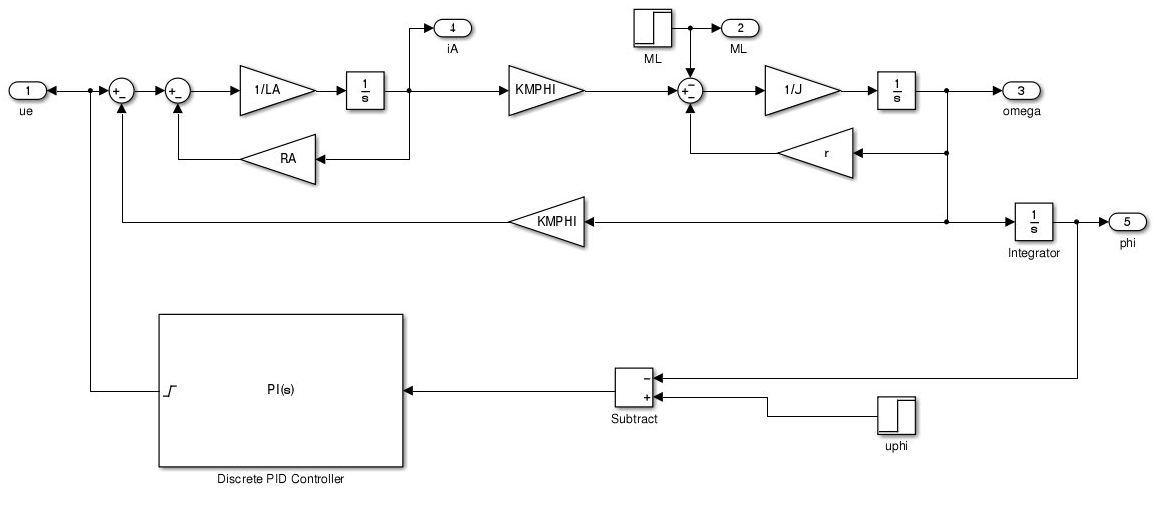
\includegraphics[width=0.6\textwidth]{sSpiegel.jpg}
	\caption{Simulink Grundprogramm}
	\label{fig:grundprogramm}
\end{figure}

\section{Matlab}
\subsection{Motor in Matlab}
Die Programmentwicklung in Matlab gestaltet sich für den Motor als relativ einfach, da, wie oben erwähnt, keien Motordaten gefunden wurden, wird auf das Matlabfile von 
Prof. Froriep aus der Vorlesung "Systemtechniken" zurück gegriffen.
In diesem Matlabfile stehen die Motorkenndaten, die berechnete Trägheit des Spiegels, das berechnete Drehmoment, die Grenzen für die Plots, Anweisungen für die Plots und
für den Integrationsalgorithmus.
Dieses File ist eine sehr gute Grundlage für die Simuation, welches während der Simulation entsprechend angepasst werden kann.

Als Größen zur Ausgabe in einem Diagramm, interessieren vor allem die Eingangsspannung $u_e$, der aktuelle Winkel $\phi$, sowie der Sollwinkel mit seinen Toleranzen.
Es werden drei Plots dargestellt.
In dem ersten Plot ist die Motorspannung dargestellt.
In dem zweiten Plot der aktuelle Winkel $\phi$, der direkt von dem Motor abgegriffen wird, sowie der einzustellende Sollwinkel dargestellt.
Der dritte Plot enthält auch wieder den aktuellen Winkel $\phi$, jedoch mit einer feineren Auflösung um den Sollwinkel, um die Toleranzgrenzen besser erkennen zu können.

\subsection{Sensor in Matlab}
Der Sensor selbst wird nur mit Matlabprogrammen simuliert.
Dies ermöglicht verschiedene Sensoren in das Hauptprogramm einzubinden und Änderungen an z.B. den Ausmaßen des Sensors vorzunehmen, ohne das Hauptprogramm ändern zu müssen.

\subsubsection{Vorbereitungen}
Um einen Sensor mit seinen verschiedenen Kenngrößen wie Sensorfläche, Übertragungsverhalten, und weiteres simulieren zu können, werden die verschiedenen Funktionen aus
Kap. \ref{chap:sensor}in einzelnen Matlabfiles gespeichert. 
Dieses macht die Aufgabenlösung zwar komplexer, bietet aber den Vorteil, einzelne Bereiche für sich testen zu können, bevor sie in den Sensor eingebunden werden.

\subsubsection{Files}
Ich würde hier evtl. schreiben, in welche Unterprogramme Du den Sensor aufgeteilt hast.
Auch sollten Deine Versuchsprogramme erwähnt und mit in den Anhang kommen.
Da steckt viel Arbeit drin und war/ist für die Simuation äußerst wichtig.